\documentclass[11pt,compress,xcolor={usenames,dvipsnames}]{beamer}
\usepackage[english]{babel}
\usepackage[T1]{fontenc}
\usepackage[]{algorithm2e}
\usepackage{caption}
\usepackage{media9}
\captionsetup[figure]{labelformat=empty}

\usepackage{changepage}


\title[Chatting Plattform]{Development of a Chatting Platform} 
\author[Synomilia]{Synomilia} 
\date[08-02-2017]{8th February 2017}
\institute[]{King's College London} 
\titlegraphic{
\includegraphics[width=30mm]{kcl-logo.jpg}}



\usetheme{Madrid} 
\useoutertheme[]{miniframes} 
%\usecolortheme[]{beaver}
%\usecolortheme{albatross}
%\usecolortheme{beaver}
%\usecolortheme{beetle}
%\usecolortheme{crane}
%\usecolortheme{dolphin}
%\usecolortheme{dove}
%\usecolortheme{fly}
\usecolortheme{lily}
%\usecolortheme{orchid}
%\usecolortheme{rose}
%\usecolortheme{seagull}
%\usecolortheme{seahorse}
%\usecolortheme{whale}
%\usecolortheme{wolverine}


%\setbeamercolor*{structure}{fg=} 

\PassOptionsToPackage{subsection=false}{beamerouterthememiniframes}
\usepackage{remreset}
\makeatletter
\@removefromreset{subsection}{section}
\makeatother
\setcounter{subsection}{1}

\makeatletter
\beamer@theme@subsectionfalse
\makeatother


%\setbeamercovered{dynamic}


\setbeamertemplate{footline}
{
  \leavevmode%
  \hbox{%
  \begin{beamercolorbox}[wd=.4\paperwidth,ht=2.25ex,dp=1ex,center]{author in head/foot}%
    \usebeamerfont{author in head/foot}\insertshortauthor
  \end{beamercolorbox}%
  \begin{beamercolorbox}[wd=.6\paperwidth,ht=2.25ex,dp=1ex,center]{title in head/foot}%
    \usebeamerfont{title in head/foot}\insertshorttitle\hspace*{3em}
    \insertframenumber{} / \inserttotalframenumber\hspace*{1ex}
  \end{beamercolorbox}}%
  \vskip0pt%
}

\setbeamertemplate{navigation symbols}{}



\begin{document}

\begin{frame} 
\maketitle 
\end{frame}


\section{Project Description}
\begin{frame}
\frametitle{Goals}
\begin{itemize}
\item Deliver client server application with clients developed for two different domains
\item Become proficient in employing testing strategies and methods
\item Gain experience collaborating as a team
\item Become au fait using version control and collaboration software
\end{itemize}
\end{frame}

\begin{frame}
\frametitle{Implementation Strategy}
\begin{itemize}
\item Background research was done on how to implement a client server system/application
\item Basic prototype was developed to understand how sockets work etc.

%\includemedia[
%  width=0.4\linewidth,
%  height=0.3\linewidth,
%  activate=onclick,
%  addresource=/Users/Sagar/AppData/Roaming/Skype/My Skype Received Files/MyMovie1.mp4,
%  flashvars={source=/Users/Sagar/AppData/Roaming/Skype/My Skype Received Files/MyMovie1.mp4}
%]{}{VPlayer.swf}

%\mediabutton[ mediacommand=some_dice:playPause, overface=\color{blue}{\fbox{\strut Play/Pause}}, downface=\color{red}{\fbox{\strut Play/Pause}}
%]{\fbox{\strut Play/Pause}} \mediabutton[
%mediacommand=some_dice:setSource [(random.mp4)] ]{\fbox{\strut random.mp4}} \mediabutton[
%mediacommand=some_dice:setSource [(cube.mp4)] ]{\fbox{\strut cube.mp4}}

\item Team will be split into three sub-teams 
\begin{itemize}
\item one team will implement the server in python 
\item another team will work on the desktop client 
\item last team will work on the android client 
\end{itemize}
\item Test plans (unit testing and regression \& integration testing)
\end{itemize}
\end{frame}

\begin{frame}
\frametitle{}
\centering
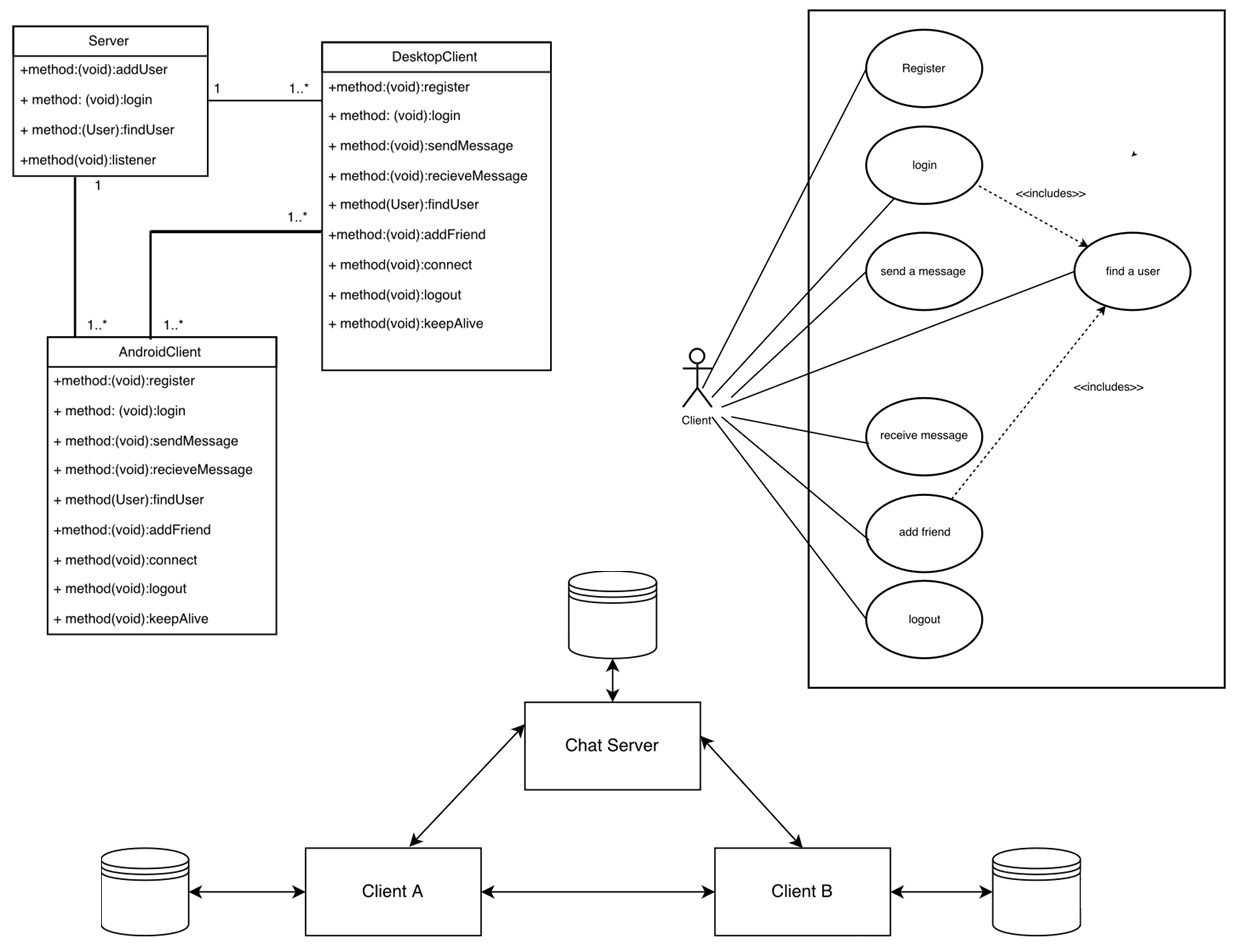
\includegraphics[scale=0.5]{UMLdiagrams.png}
\end{frame}

\begin{frame}
\frametitle{Timeline - Mandatory Features}
\begin {table}[H]
\begin{center}
\begin{tabular}{|c|c|}
\hline 
\rule[-1ex]{0pt}{2.5ex} \textbf{Deadlines} & \textbf{Mandatory Feature List} \\ 
\hline 
\rule[-1ex]{0pt}{2.5ex} 18/02 & Send text based messages to one or more users \\ 
\hline 
\rule[-1ex]{0pt}{2.5ex} 18/02 & Receive text based messages from one or more users \\ 
\hline 
\rule[-1ex]{0pt}{2.5ex} 18/02 & Secure communication between users \\ 
\hline 
\rule[-1ex]{0pt}{2.5ex} 25/02 & Search for other users on the server \\ 
\hline 
\rule[-1ex]{0pt}{2.5ex} 25/02 & User Registration (New User) \\ 
\hline 
\rule[-1ex]{0pt}{2.5ex} 25/02 & User authentication (Log in/Log out) \\ 
\hline 
\rule[-1ex]{0pt}{2.5ex} 04/03 & Chat client for mobile \\ 
\hline 
\rule[-1ex]{0pt}{2.5ex} 04/03 & Chat client for desktop \\ 
\hline 
\end{tabular} 
\end{center}
\end {table}
\end{frame}

\begin{frame}
\frametitle{Optional Features}
With accordance to time availability, optional features can be added.

\begin {table}[H]
\begin{center}
\begin{tabular}{|c|c|}
\hline 
\multicolumn{2}{|c|}{\textbf{Optional Feature List}}\\
\hline 
\rule[-1ex]{0pt}{2.5ex} Set Status & Emojis \\ 
\hline 
\rule[-1ex]{0pt}{2.5ex} Send Images or Files & Backup Chat/Chat Log \\ 
\hline 
\rule[-1ex]{0pt}{2.5ex} Set name/Profile Picture & Remove messages \\ 
\hline 
\rule[-1ex]{0pt}{2.5ex} Delete user account & Chat time stamps  \\ 
\hline 
\rule[-1ex]{0pt}{2.5ex} Contact List  & Customised Chat background  \\ 
\hline 
\end{tabular} 
\end{center}
\end {table}
\end{frame}

\begin{frame}
\begin{center}
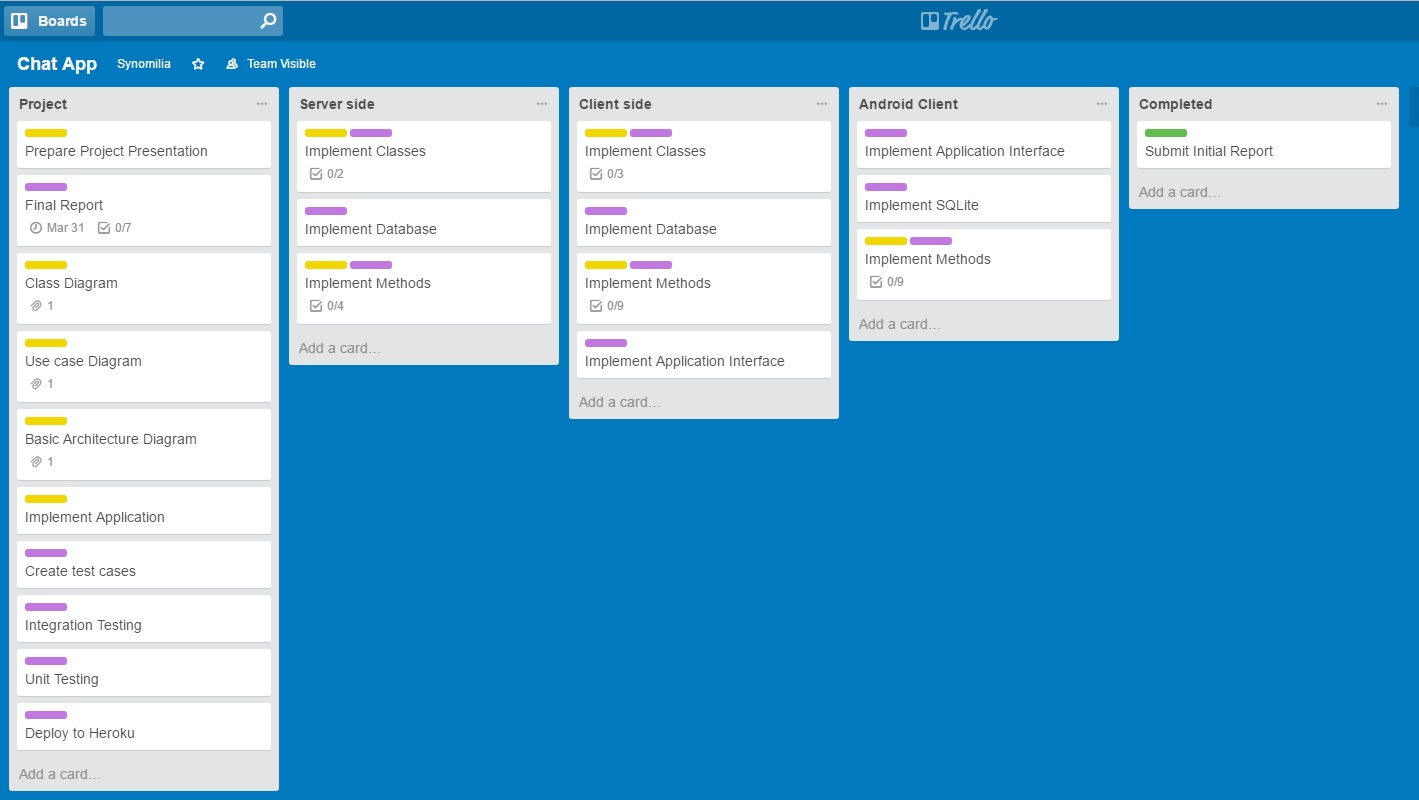
\includegraphics[scale=0.3]{trelloboard.jpg}

\end{center}\end{frame}

 
\section{Project Organization}
\begin{frame}
\frametitle{Working Together as a Team}
\begin{itemize}
\item Initial kick-off meeting and general brainstorming
\item Physical meetings are held every Tuesday at 5pm
\item Development meetings will be organised at periodic intervals
\item Skype/virtual meetings will be organised on-demand 
\item WhatsApp group for instant communication
\end{itemize}
\end{frame}

\begin{frame}
\frametitle{Conflicts Resolution}
Peer assessment: equal distribution of marks

Few of the potential sources of conflicts could be:
\begin{itemize}
\item Difference of opinions on prioritization
\item Technical and design disagreements
\item Disagreements on schedule or timeline
\item Lack of consensus on unified process methodologies
\end{itemize}
Few solutions that we expect to adopt are:
\begin{itemize}
\item Mutual cooperation and taking ownership of any proposed idea
\item Having a consensus on the decision taken by the group and abiding by it
\end{itemize}
\end{frame}

\end{document}